\section{Indeksowanie tekstu}

\begin{algorithm}[H]
    \caption{Indeksowanie tekstu}
    \Input{Słowo $t \in \A^+$ ($|t| = n$)}
    \Output{Struktura danych, na której można wykonywać zapytania \emph{czy $w$ jest podsłowem $t$} dla dowolnego $w \in \A^*$ ($|w| = m)$.}
\end{algorithm}

Typowo zakładamy, że $m \ll n$ oraz wymagamy, aby zapytanie było wykonywalne w czasie $O(m)$, niezależnym od $n$. Czasem dopuszczamy, aby czas wykonania zapytań był logarytmiczny względem $n$.

Dodatkowo wstępne przetwarzanie tekstu powinno było wykonalne w czasie liniowym lub przynajmniej liniowo-polilogarytmicznym względem $n$ (oraz rozmiaru alfabetu $\A$).

\subsection{Drzewo sufiksowe}

Drzewo sufiksowe (\emph{suffix trie}) to jedna ze struktur danych, która umożliwia łatwe sprawdzanie podsłów. W najprostszej, nieskompresowanej wersji jest to zwykłe drzewo słownikowe $Trie(t)$ zawierające wszystkie sufiksy słowa $t$.

%Słowo: aabbabbc
\begin{center}
\includegraphics[width=0.45\linewidth]{graphics/suffix-trie-example.png}
\end{center}

Sprawdzenie, czy słowo $w$ jest podsłowem $t$ polega po prostu na sprawdzeniu, czy w drzewie sufiksowym $Trie(t)$ istnieje ścieżka zgodna z kolejnymi literami słowa $w$.

Pewnym ułatwieniem rozważań na drzewach sufiksowych jest zastosowanie specjalnego znaku $\$ \notin \A$ na końcu $t$. W ten sposób zapewniamy, że każdy sufiks $t$ kończy się w liściu tj. żaden sufiks nie jest prefiksem innego sufiksu.

\begin{problem}{}{}
  Dla dowolnego $n$ pokaż tekst $t$ długości $n$ taki, że rozmiar drzewa sufiksowego jest możliwie największy.
\end{problem}

% Słowo: a^n b^n a^n b^n c

Ponieważ podstawowe drzewo sufiksowe może mieć rozmiar większy niż liniowy, to wygodniejsze jest przejście na skompresowane drzewo sufiksowe (\emph{suffix tree}) $ST(t)$ tj. drzewo, w którym ściągnięto wszystkie wierzchołki stopnia $2$ różne od korzenia. Każda krawędź w drzewie zamiast odpowiadać pojedynczej literze, odpowiada teraz pewnemu słowu z $\A^+$. Dowolne dwie krawędzie wychodzące z tego samego wierzchołka odpowiadają słowom, których największych prefiks jest pusty (tj. różnią się pierwszym znakiem).
Oczywiście sprawdzenie, czy $w$ jest podsłowem $t$ przebiega dokładnie tak samo jak poprzednio.

\begin{theorem}{}{}
  Skompresowane drzewo sufiksowe dla dowolnego słowa $t$ o długości $n$ ma rozmiar $O(n)$.
\end{theorem}

\begin{proof}
  Wiemy, że drzewo $ST(t)$ ma co najwyżej $n$ liści (jeśli kończy się symbolem specjalnym, to ma dokładnie $n$). Z definicji każdy wierzchołek wewnętrzny drzewa skompresowanego ma co najmniej dwa poddrzewa, wobec tego liczba wierzchołków wewnętrznych musi być mniejsza od liczby liści.
\end{proof}

Z powyższych twierdzeń jasne jest, że konstrukcja skompresowanego drzewa sufiksowego przez najpierw zbudowanie, a następnie kompresję drzewa nieskompresowanego jest nieoptymalna.

% TODO s. 84-85 w crochermore1994text -- algorytmy naiwne

Optymalne podejścia przedstawione poniżej polegają na iteracyjnym rozbudowywaniu drzewa sufiksowego przez wstawianie kolejnych sufiksów we właściwej kolejności, od najdłuższego lub od najkrótszego. Okazuje się, że samo to jednak nie wystarczy:
\begin{problem}{}{}
  Dla dowolnego $n$ pokaż tekst $t$ ($|t| = n$) taki, że wstawianie sufiksów do drzewa sufiksowego w dowolnej kolejności zaczynając zawsze od korzenia wymaga $\Theta(n^2)$ operacji.
\end{problem}

\subsubsection{Algorytm McCreighta}

W omawianiu algorytmów będziemy korzystać oznaczenia $ST(t, i)$ jako (tymczasowego) drzewa słownikowego, zawierającego $i$ najdłuższych sufiksów $t$. Oznaczmy przez $leaf(i)$ liść wstawiony przy przejściu z $ST(t, i - 1)$ do $ST(t, i)$, odpowiadający sufiksowi $t[i..n]$. Dodatkowo, $head(i) = parent(leaf(i))$.

Ponadto, zdefiniujmy dla każdego wierzchołka $v$ funkcję $word(v)$ przypisującą mu słowo złożone z etykiet ścieżki od korzenia do $v$.
Jest to szczególnie użyteczne do definicji linków sufiksowych, wykorzystywanego w algorytmie: jeśli $word(v) = aw$ ($a \in \A$, $w \in \A^*$), to $S[v] = u$, gdzie $u$ jest wierzchołkiem, dla którego $word(u) = w$.

\begin{code}
\captionof{listing}{Algorytm McCreighta budowania drzewa sufiksowego}
\inputminted{python}{code/suffix-tree/mccreight.py}
\label{alg:mccreight-suffix-tree}
\end{code}

W dowodzie optymalności algorytmu McCreighta wykorzystywane będą następujące trzy własności:
\begin{problem}{crochemore1994text}{s. 91}
  Pokaż, że $head(i)$ jest potomkiem $S[head(i - 1)]$ w $ST(t, i)$.
\end{problem}

\begin{problem}{crochemore1994text}{s. 91}
  Pokaż, że $S[v]$ jest potomkiem $S[parent(v)]$ dla dowolnego $v$ w każdym $ST(t, i)$.
\end{problem}

\begin{problem}{}{}
  Pokaż, że $depth(v) \le depth(S[v]) + 1$ dla dowolnego $v \neq head(i)$ w każdym $ST(t, i)$.
\end{problem}

\begin{theorem}{}{}
  Algorytm McCreighta zwraca poprawne drzewo sufiksowe.
\end{theorem}

\begin{proof}
  Na początek załóżmy, że dla dowolnego $i = 2, 3, \ldots, n$ mamy zbudowane $ST(t, i - 1)$ oraz wszystkie wierzchołki wewnętrzne $ST(t, i - 1)$ inne niż $head(i - 1)$ mają dobrze zdefiniowane $S[v]$ (samo $S[head(i - 1)]$ też może być zdefiniowane wcześniej, ale nie musi). Ten niezmiennik jest utrzymany przez cały algorytm.

  Oczywiście $ST(t, 1)$ złożone z korzenia $r$, liścia $l_1$ i krawędzi między nimi z etykietą $t$ spełnia te warunki.
  
  Korzystając obu własności z problemów powyżej wiemy, że $S[parent(head(i - 1)]$ jest dobrze zdefiniowany oraz istnieje ścieżka z $S[parent(head(i - 1)]$ do $S[head(i - 1)]$ w $ST(t, i - 1)$ -- jedynie z tym zastrzeżeniem, że może kończyć się ,,w środku'' krawędzi tj. z $head(i - 1)$ jako wierzchołkiem skompresowanym.
  
  Wystarczy zatem dodać wierzchołek $leaf(i)$, być może rozbijając krawędź i tworząc nowy wierzchołek $head(i - 1)$, oraz nadać wartość $S[head(i - 1)]$ tak, żeby $S[head(i - 1)]$ było przodkiem $head(i)$, aby stworzyć drzewo, które jest $ST(t, i)$ oraz ma dobrze zdefiniowane $S[v]$ dla wszystkich wierzchołków wewnętrznych $v$ poza $head(i)$.
\end{proof}

\begin{theorem}{}{}
  Algorytm McCreighta ma złożoność $O(n \log{|\A|})$.
\end{theorem}

\begin{proof}
  Złożoność czasowa algorytmu wynika wprost z trzech faktów.
  
  Po pierwsze, poza funkcjami \texttt{fast\_find} i \texttt{slow\_find} algorytm wykonuje stałą liczbę operacji w każdej iteracji -- a zatem $O(n)$ operacji łącznie.
  Dla alfabetu $\A$ znalezienie w wierzchołku odpowiedniej krawędzi zaczynającej się od danego symbolu wynosi $O(\log{|\A|})$. Wszystkie pozostałe operacje wykonywane są w czasie stałym.

  Po drugie, niech funkcja \texttt{fast\_find} schodzi od wierzchołka $S[parent(head(i - 1))]$ w dół do wierzchołka $head(i)$ po dokładnie $d_i$ krawędziach. Wówczas wiemy, że
  \begin{align*}
    depth(head(i - 1)) \le depth(S[head(i - 1)]) + 1 = depth(head(i)) - d_i + 1.
  \end{align*}
  Wobec tego całkowita liczba przejść po krawędziach w funkcji \texttt{fast\_find} wynosi
  \begin{align*}
    \sum_{i = 2}^{n + 1} d_i \le \sum_{i = 2}^{n + 1} \left(depth(head(i)) - depth(head(i - 1)) + 1\right) \le depth(head(n)) + n \le 2 n
  \end{align*}

  Po trzecie, funkcja \texttt{slow\_find} w $i$-tej iteracji algorytmu wykonuje $s_i$ porównań, gdzie zachodzi $s_i \le |word(head(i))| - |word(head(i - 1))|$. Analogicznie jak powyżej, łączna liczba operacji jest ograniczona z góry przez $O(n)$.
\end{proof}

Warto zauważyć, że jeśli $S[head(i - 1)]$ jednak jest dobrze określone w $i$-tym kroku algorytmu, to możemy od razu przejść do tego wierzchołka, zamiast wykonywać przejście przez rodzica $head(i - 1)$ (tzw. \emph{up-link-down}). Taka optymalizacja nie zmienia jednak asymptotycznego czasu wykonania algorytmu.

\begin{problem}{crochemore1994text}{s. 93-94}
  Pokaż, że jeśli w Algorytmie \ref{alg:mccreight-suffix-tree} zamiast \texttt{fast\_find} użylibyśmy funkcji \texttt{slow\_find}, to dla dowolnego $n$ istnieje tekst $t$ długości $n$ taki, że konstrukcja $ST(t)$ wymaga czasu $\Omega(n^2)$.
\end{problem}

% Przykład: a^n

\subsubsection{Algorytm Ukkonena}

Algorytm Ukkonena polega na tym, że w tym przypadku budowane jest w zasadzie poprawne drzewo sufiksowe dla kolejnych prefiksów słowa $t$.
W trakcie wykonania algorytmu wyznaczamy dokładnie taką samą tablicę linków sufiksowych jak w algorytmie McCreighta.

\begin{code}
\captionof{listing}{Algorytm Ukkonena budowania drzewa sufiksowego}
\inputminted{python}{code/suffix-tree/ukkonen.py}
\label{alg:ukkonen-suffix-tree}
\end{code}

\begin{problem}{}{}
  Pokaż, że wartości $S[v]$ wyznaczane w algorytmach McCrieghta i Ukkonena są identyczne.
\end{problem}

\begin{theorem}{}{}
  Algorytm Ukkonena zwraca poprawne drzewo sufiksowe.
\end{theorem}

\begin{proof}
  Przede wszystkim zauważmy, że każdy nowododany liść pozostaje zawsze liściem do samego końca wykonania algorytmu -- w ten sposób $leaf(i)$ nie tylko reprezentuje sufiks $t[i]$ w $ST(t, i)$, ale również sufiks $t[i..j]$ w $ST(t, j)$ dla dowolnego $j \ge i$.
  
  Należy przy tym pamiętać, że w rzeczywistości, inaczej niż w powyższym algorytmie, pamiętamy nie całą etykietę na krawędzi, tylko parę liczb oznaczających początek i koniec etykiety w tekście. Wystarczy zatem ustawić indeksy końcowe w liściach na $+\infty$, unikając w ten sposób problemu z dodawaniem kolejnych znaków na końcach liści.
  
  Aby z $ST(t, i - 1)$ otrzymać $ST(t, i)$ wystarczy wstawić do drzewa wszystkie sufiksy słowa $t[1..i]$. Załóżmy jednak, że pewnym momencie natrafimy na (być może skompresowany) wierzchołek $v$, dla którego już istnieje (być może skompresowany) wierzchołek $v'$ spełniający $word(v) = word(v') \, t[i]$. Wówczas wiemy, że w drzewie nieskompresowanym dla wszystkich wierzchołków $u$ odpowiadających sufiksom słowa $word(v)$ istnieją wierzchołki $u'$ takie, że $word(u) = word(u') \, t[i]$. Wobec tego wszystkie mniejsze sufiksy słowa $t[1..i]$ już muszą istnieć.
  
  Idea algorytmu jest zatem taka: w $i$-tej iteracji wychodzimy od $head(i - 1)$ (zob. dowód algorytmu McCreighta) i chodząc po linkach sufiksowych rozbudowujemy drzewo o nowe liście zgodnie z $t[i]$ aż do momentu, gdy natrafimy na istniejący (może skompresowany) wierzchołek. Tak otrzymane drzewo (gdybyśmy zastąpili wszystkie indeksy końcowe $+\infty$ przez $i$) jest drzewem sufiksowym $ST(t, i)$.
\end{proof}

\begin{theorem}{}{}
  Algorytm Ukkonena ma złożoność $O(n \log{|\A|})$.
\end{theorem}

\begin{proof}
  Wszystkie operacje poza \texttt{fast\_find} wymagają czasu $O(\log{|\A|})$ na każdą iterację głównej pętli.
  
  Pętla \texttt{while} za każdym razem dodaje jeden liść, więc podczas całego wykonania algorytmu funkcja \texttt{fast\_find} zostanie wykonana $O(n)$ razy.
  Ponieważ wiemy, że $S[v]$ przyjmuje dokładnie takie same wartości, jak w algorytmie McCreighta, to również tu całkowita liczba odwiedzionych wierzchołków w funkcji \texttt{fast\_find} wyniesie $O(n)$.
\end{proof}

\subsubsection{Dalsze zagadnienia}

\citet{giegerich1997ukkonen} pokazali, że chociaż teoretyczne idee u podstaw wszystkich trzech algorytmów się różnią, to istnieje głębokie podobieństwo strukturalne. W szczególności można pokazać, że algorytmy McCreighta i Ukkonena wykonują dokładnie te same ciągi abstrakcyjnych operacji, a zatem możliwe jest tłumaczenie krok po kroku wykonania jednego algorytmu na drugi. Również algorytm Weinera przypomina strukturalnie algorytm Ukkonena z tą różnicą, że jest budowany ,,od końca'' i przez to korzysta jedynie z ,,przybliżonych'' linków.

Okazuje się, że możliwa jest konstrukcja drzewa sufiksowego w czasie $O(n)$, niezależnym od $\A$ \citep{farach1997optimal}. Wymaga to co prawda utożsamienia alfabetu z podzbiorem liczb naturalnych zamiast z dowolnym zbiorem z liniowym porządkiem, ale w przeciwieństwie do sortowania nie stanowi żadnego problemu.

Drzewa sufiksowe umożliwiają nie tylko szybkie obliczanie zapytań o przynależność, ale mogą również służyć do rozwiązywania kilku innych problemów.

\begin{problem}{crochemore2002jewels}{Theorem 5.2, s. 59-60}
  Pokaż, jak w czasie $O(m)$ odpowiadać na zapytania, ile razy słowo $w$ ($|w| = m$) występuje w tekście $t$, gdy mamy skonstruowane $ST(t)$.
\end{problem}

\begin{proof}
Mając zbudowane drzewo sufiksowe, idziemy od korzenia w dół czytając kolejne symbole $w$, a czasami posuwamy się po wewnętrznej etykiecie pewnej krawędzi. Wówczas zbiór wystąpień odpowiada zbiorowi liści w poddrzewie węzła, do którego udało nam się w ten sposób dojść. Liczbę takich liści możemy ustalić bardzo łatwo: budując drzewo sufiksowe możemy od razu obliczyć w każdym węźle trzymać ile liści jest w jego poddrzewie. Jeżeli po drodze nie dało się dalej schodzić po drzewie, oznacza to, że $w$ nie jest podsłowem słowa $t$, więc odpowiedzią jest zero.
\end{proof}

\begin{problem}{crochemore2002jewels}{Lemma 5.1, s. 63}
  Pokaż, jak w czasie $O(n)$ policzyć, ile różnych podsłów zawiera słowo $t$ ($|t| = n$).
\end{problem}

\begin{proof}
Gdybyśmy zbudowali takie pełne drzewo sufiksowe bez kompresji, to wówczas jest to po prostu drzewo trie wszystkich sufiksów danego słowa. Wówczas liczba różnych podsłów słowa $n$ jest po prostu równa liczbie wierzchołków w stworzonym drzewie. W przypadku, gdy budujemy drzewo sufiksowe z kompresją, aby nie mieć kwadratowego rozmiaru całej struktury, należy również policzyć wierzchołki w zbudowanym drzewie, ale dodatkowo licząc wierzchołki liczymy je z odpowiednimi wagami, które wynikają z tego, że wierzchołki w skompresowanym drzewie sufiksowym są tak naprawdę ścieżkami wierzchołków i je też należy uwzględnić, co możemy zrobić bardzo łatwo, poprzez popatrzenie jakie etykiety są trzymane w wierzchołkach i dodając odpowiednie krotności. Możemy to wszystko zrobić jednym przejściem po drzewie, skąd wynika liniowa złożoność względem długości słowa.
\end{proof}

\begin{problem}{crochemore2002jewels}{Theorem 5.3, s. 62}
  Pokaż, jak w czasie $O(n k)$ wyznaczyć najdłuższe wspólne podsłowo dla zbioru słów $\{t_i: 1 \le i \le k\}$ długości co najwyżej $n$.
\end{problem}

\begin{proof}
Rozwiązanie jest oczywiście bardzo proste. Wystarczy zbudować drzewo sufiksowe, ale nie dla każdego słowa osobno, ale jedno wspólne. Robimy to w ten sposób, że najpierw budujemy drzewo sufiksowe dla pierwszego słowa. Następnie wstawiamy do niego sufiksy drugiego słowa, trzeciego itd aż do $k$-tego, z tą różnicą, że wstawiając słowa, w wierzchołkach pamiętamy sobie informacje jaki sufiks tędy przechodzi w dół, tzn. każdy wierzchołek ma informacje na temat tego, sufiksy którego słowa przez niego przechodziły. Wówczas odpowiedzią, czyli najdłuższym wspólnym podsłowem, będzie najgłębiej położony węzeł w naszym drzewie zbudowanym dla $n$ słów, przez który przeszedł jakiś sufiks każdego słowa. Oczywiście można tego LCSa bardzo łatwo odtworzyć jak już mamy taki najgłębszy wierzchołek o tej własności. Wystarczy przejść się od korzenia do niego i zobaczyć jakie etykiety mijaliśmy po drodze.
\end{proof}

\subsubsection{Algorytm Weinera}

Algorytm Weinera, historycznie najwcześniejszy algorytm optymalny, polega na budowaniu drzewa sufiksowego od prawej do lewej. Zauważmy, że dzięki przeglądaniu tekstu w tej kolejności gwarantujemy, że w $i$-tym kroku budowana struktura danych jest pełnoprawnym drzewem sufiksowym dla słowa $t[(n - i - 1)..n]$.

Tak jak w algorytmie McCreighta, najważniejszą częścią algorytmu jest efektywne wyznaczanie linków między wierzchołkami drzewa -- z tą różnicą, że w tym przypadku są to linki odwrotne do linków sufiksowych.
Definiujemy je następująco: jeśli $word(v) = w$ ($w \in \A^*$) oraz $t[i] = a$, to $link_a[v] = u$, gdzie $u$ jest pewnym wierzchołkiem, dla którego $word(u) = a \, word(v)$.

Niniejsza implementacja jest oparta na uproszczonej wersji algorytmu, zamieszczonej w \citet{breslauer2013near}.
\begin{code}
\captionof{listing}{Algorytm Weinera budowania drzewa sufiksowego}
\inputminted{python}{code/suffix-tree/weiner.py}
\label{alg:suffix-tree-weiner}
\end{code}

\begin{problem}{}{}
  Pokaż, że Algorytm \ref{alg:suffix-tree-weiner} wyznacza w każdej iteracji poprawne przejścia $link[v, c] = u$.
\end{problem}

\begin{problem}{}{}
  Pokaż, że Algorytm \ref{alg:suffix-tree-weiner} zwraca poprawne drzewo sufiksowe.
\end{problem}

\begin{problem}{}{}
  Pokaż, że Algorytm \ref{alg:suffix-tree-weiner} działa w czasie $O(n \log{|\A|})$.
\end{problem}

\subsection{Tablica sufiksowa}

Tablica sufiksowa jest dużo prostszą strukturą, wprowadzoną jako alternatywa dla drzew sufiksowych równolegle w \citep{gonnet1992new} i \citep{manber1993suffix}.
Wartości tablicy dla słowa $t$ długości $n$ definiujemy następująco:
\begin{align*}
    SA[i] = |\{j: t[j..n] \le t[i..n]\}|,
\end{align*}
czyli na $i$-tej pozycji mamy początkowy indeks $i$-tego najmniejszego sufiksu w porządku leksykograficznym.

Naiwny algorytm liczenia tablicy $SA$ wymaga czasu $O(n^2 \log{n})$, gdy wykorzystujemy sortowanie wymagające $O(n \log{n})$ porównań, ponieważ każde porównanie wymaga w najgorszym przypadku czasu $O(n)$.

Można również obliczyć tablicę $SA$ na podstawie zadanego drzewa sufiksowego w czasie $O(n)$: wystarczy przejrzeć drzewo wgłąb lub rekurencyjnie zgodnie z kolejnością liter w alfabecie. Zwróćmy uwagę, że Algorytm \ref{alg:suffix-array-from-suffix-tree} wyznacza długości słów na podstawie znajomości tekstu i aktualnej głębokości przeszukiwania.

\begin{code}
\captionof{listing}{Algorytm budowania tablicy sufiksowej na podstawie drzewa sufiksowego}
\inputminted{python}{code/suffix-array/from-suffix-tree.py}
\label{alg:suffix-array-from-suffix-tree}
\end{code}


    \subsection{Cel algorytmu i format wejścia}
    Wejściem do algorytmu jest słowo $w$ o długości $n$ nad alfabetem $\Sigma = [n]$ - liczb naturalnych od $1$ do $n$. Zakładać będziemy, że $n = 2^k$ - jeśli nie, to można słowo $w$ wydłużyć o czynnik liniowy, tak żeby ta równość zachodziła, dodając na koniec odpowiednią ilość $'\$'$, a po wykonaniu algorytmu ``uciąć'' z drzewa sufiksowego poddrzewa odpowiadające tym symbolom. \\ \\
    Algorytm tworzy drzewo sufiksowe dla tego słowa w czasie $O(n)$. Od drzewa wymagane jest, aby dla każdego wierzchołka, krawędzie prowadzące do jego dzieci posortowane były leksykograficznie względem ich etykiet (w przypadku liczb naturalnych porządek leksykograficzny rozumiemy jako zdefiniowany przez zwykłą relację $<$).
    
    \subsection{Idea algorytmu}
    Algorytm Faracha działa rekurencyjnie i każdy jego etap można zapisać w trzech krokach:
    \begin{enumerate}
     \item Zbuduj drzewo sufiksowe $T_o$ dla \textit{nieparzystych} sufiksów, czyli takich, które zaczynają się od nieparzystego indeksu (numerujemy od $1$).
     \item Korzystając z drzewa $T_o$, zbuduj drzewo $T_e$ - drzewo sufiksowe dla \textit{parzystych} sufiksów (bez wywołania rekurencyjnego!).
     \item Połącz drzewa $T_o$ i $T_e$ w jedno drzewo $T$.
    \end{enumerate}
    Jeśli kroki $2.$ i $3$ będziemy w stanie wykonać w liniowej złożoności, to wówczas cały algorytm będzie miał złożoność:
    $$
        T(n) = T\left(\frac{n}{2}\right) + O(n),
    $$
    a więc liniową. \\
    Aby  uniknąć dodatkowego wywołania rekurencyjnego w równaniu (co zwiększyłoby złożoność do $O(nlgn)$), drzewo $T_e$ konstruowane będzie bezpośrednio z drzewa $T_o$.
    
    \subsection{Tworzenie drzewa $T_o$}
    Tworzenie drzewa nieparzystych sufiksów przebiega w kilku krokach:
    \begin{enumerate}
     \item $\forall i \in [\frac{n}{2}]$ stwórz parę $\langle w[2i-1], w[2i] \rangle$ i wszystkie takie pary umieść w liście $S'$ i każdą z nich zamień na jej \textit{rangę} (indeks w posortowanej leksykograficznie liście). Na przykład, dla słowa \verb|121112212221|, lista $S'$ wygląda tak: \\
     \verb|[(1,2), (1,1), (1,2), (2,1), (2,2), (2,1), #]|, a po zamianie elementów na ich rangi, tak: \\
     \verb|[2,1,2,3,4,3,#]|.
     \item Rekurencyjnie oblicz $T_{S'}$ - drzewo sufiksowe dla słowa $S'$ oraz jego tablicę sufiksową składającą się z $A_{T_{S'}}$ - posortowanej tablicy sufiksów i z $LCP_{T_{S'}}$ - tablicy najdłuższych wspólnych prefiksów dla $A_{T_{S'}}$.
     \item Korzystając z $A_{T_{S'}}$, oblicz $A_{T_o}$ w następujący sposób:
     $$
        A_{T_o}[i] = 2A_{T_{S'}}[i] - 1,
     $$
     co bazuje na obserwacji, że każdy nieparzysty sufiks $w[2i-1]...w[n]$ jest równoważny sufiksowi $S'[i]...S'[\frac{n}{2}]$ (co wynika z konstrukcji $S'$), a zatem leksykograficzny porządek $A_{T_{S'}}$ jest taki sam jak porządek $A_{T_o}$. Jedyne co trzeba zmienić, to indeksy, odwracając przekształcenie z punktu $1.$: $\langle w[2i-1],w[2i] \rangle \rightarrow S'[i]$.
     \item Oblicz $LCP_{A_{T_o}}$, korzystając z $LCP_{A_{T_{S'}}}$, według wzoru:
      \begin{align*}
      \left.
       LCP_{T_o}[i] = 2LCP_{T_{S'}}[i] + \bigg\{
       \begin{array}{@{}l}
        1 \text{ if } w[A_{T_o}[i] + 2LCP_{T_{S'}}] = w[A_{T_o}[i+1] + 2LCP_{T_{S'}}[i]]   \\
        0 \text{ otherwise}
       \end{array},
        \right.              
      \end{align*}
      co również wynika z konstrukcji słowa $S'$.
    \item Na podstawie $A_{T_O}$ i $LCP_{T_o}$ skonstruuj drzewo $T_o$.
    \end{enumerate}
    \subsection{Tworzenie drzewa $T_e$}
    \begin{enumerate}
     \item Wstępnie przetwórz drzewo $T_o$ (w czasie liniowym od jego rozmiaru) tak aby dało się odpowiadać na zapytania o \verb|lca| na tym drzewie w czasie stałym.
     \item Korzystając z obserwacji, że każdy parzysty sufiks to nieparzysty sufiks poprzedzony jednym znakiem, stwórz $A_{T_e}$. W tym kroku możemy wykorzystać obliczoną już listę $A_{T_o}$, ``dokleić'' odpowiedni znak przed każdym elementem $A_{T_o}$ i użyć sortowania pozycyjnego tylko dla tego pierwszego znaku.
     \item Oblicz tablicę $LCP_{T_e}$ korzystając z zapytań o \verb|lcp(word(a),word(b))|, czyli zapytań o \verb|lca(a,b)| w drzewie sufiksowym:
      \begin{align*}
      \left.
       lcp(w[2i,n],w[2j,n]) = \bigg\{
       \begin{array}{@{}l}
        lcp(w[2i+1,n],w[2j+1,n]) + 1 \text{ if } w[2i] = w[2j]   \\
        0 \text{ otherwise}
       \end{array},
        \right.              
      \end{align*}
      
      \item Stwórz $T_e$ w oparciu o $A_{T_e}$ i $LCP_{T_e}$.
    \end{enumerate}
    
\subsection{Łączenie drzew $T_o$ i $T_e$}
Zauważmy, że aby stworzyć drzewo $T$ z drzew $T_o$ i $T_e$, wystarczy zbudować tablice $A_T$ i $LCP_T$. Do uzyskania tych tablic potrzebujemy móc szybko (w czasie stałym) odpowiadać na pytania o najdłuższy wspólny prefiks dwóch sąsiadujących sufiksów w tablicy $A_T$. Umożliwiającą nam to wyrocznię uzyskamy poprzez \textit{zachłanne} połączenie drzew $T_o$ i $T_e$. \\ \\
\textit{Zachłanne} połączenie $T'$ rozumiemy jako takie połączenie dwóch drzew ($T_e$ i $T_o$), w którym:
\begin{itemize}
 \item Każdy wierzchołek z tych drzew ma odpowiadający sobie wierzchołek w drzewie $T'$, a ponadto, jeśli $e \in T_e$, $o \in T_o$ i \verb|word(e) = word(o)|, to wierzchołkom $e$ i $o$ odpowiada ten sam wierzchołek $t \in T$. \\
 Wierzchołek $u$ \textit{odpowiada} wierzchołkowi $v \in T_o \vee v \in T_e$ wtedy i tylko wtedy gdy $|word(u)| = |word(v)|$, a ponadto dla każdego wierzchołka $a$ z $T_o$ (lub $T_e$), który jest na drodze z korzenia do wierzchołka $v$ zachodzi:
 \begin{align*}
     word(v)[|word(a)| + 1] = word(u)[|word(a)| + 1],
 \end{align*}
 czyli $word(v)$ i $word(u)$ są tej samej długości i zgadzają się przynajmniej na indeksach, które odpowiadają pierwszym znakom na każdej krawędzi na drodze z korzenia do $v$.
 \item Z każdego wierzchołka $t \in T$, dla dowolnych dwóch etykiet $w$, $v$ krawędzi z niego wychodzących zachodzi: $w[0] \ne v[0]$ ($w[1] \ne v[1]$ przy numeracji od $1$).
 \item Drzewo $T'$ nie zawiera żadnych innych wierzchołków.
\end{itemize}
W skrócie można powiedzieć, że $T'$ to drzewo, które powstaje dokładnie w ten sposób co naiwnie wykonane poprawne połączenie $T_o$ i $T_e$ do $T$, z tą tylko różnicą, że zamiast porónywać wszystkie znaki na odpowiednich krawędziach (powiedzmy $u$ i $v$) (i ewentualnie dzielić je jeśli różnią się na jakiejś pozycji), porównujemy tylko pierwsze znaki, a podział robimy tylko w miejscu, w którym skończy się krótsza z nich. Procedurę tworzenia $T'$ (czyli ``nałożenia na siebie'' drzew $T_o$ i $T_e$ patrząc tylko na pierwszy znak krawędzi) przedstawia poniższy rysunek:
\begin{center}
 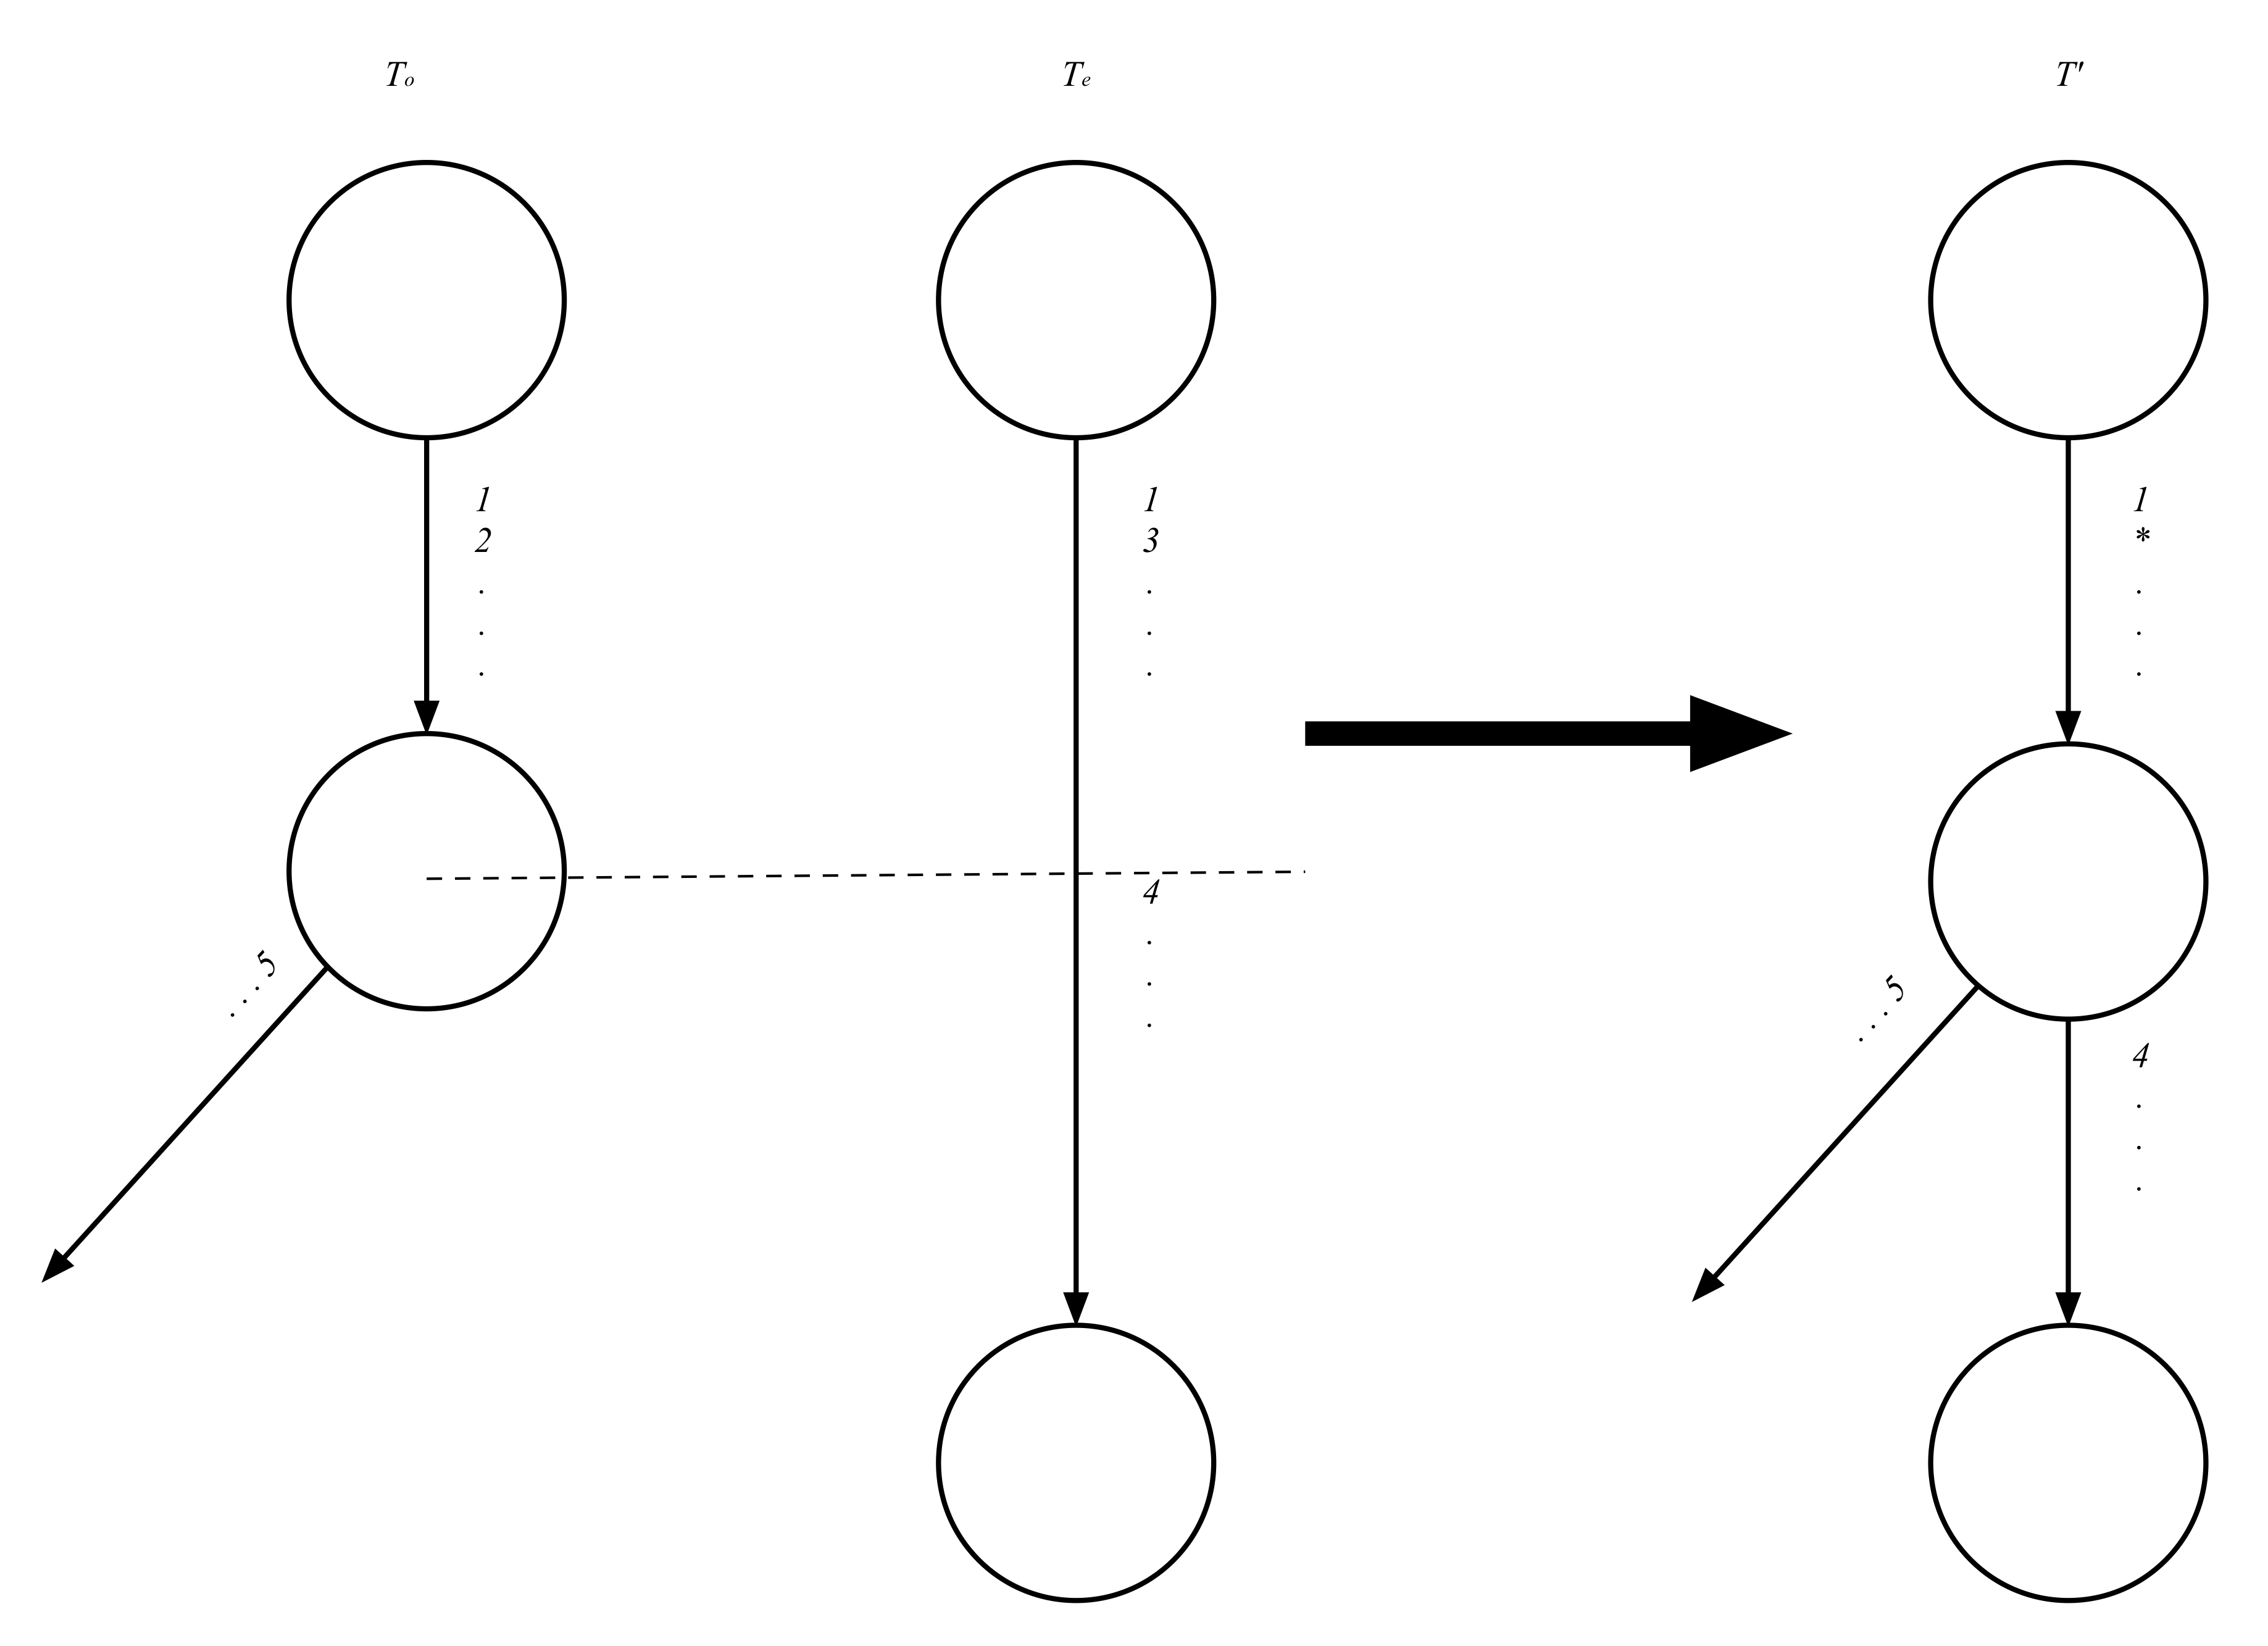
\includegraphics[scale=0.1,keepaspectratio=true]{graphics/farach-suffix-tree-overmerging.jpg}
 % overmergingSuffixTrees.jpg: 3674x2666 px, 72dpi, 129.61x94.05 cm, bb=0 0 3674 2666
\end{center}


Wiedząc jak jest konstruowane drzewo $T'$, zapiszmy kroki do stworzenia poprawnego drzewa $T$:
\begin{enumerate}
 \item Stwórz $T'$ tak jak zostało to wyżej opisane.
 \item Wierzchołek drzewa $T'$, który ma odpowiadający wierzchołek w $T_o$ nazwijmy \textit{nieparzystym}, a jeśli ma odpowiadający wierzchołek w $T_e$, to nazwijmy go \textit{parzystym}. Pewne wierzchołki (np. korzeń) mogą być zarówno parzyste jak i nieparzyste.\\
 Teraz, dla każdego wierzchołka $u \in T'$ znajdź parę wierzchołków (jeśli istnieje) $(a,b)$, które są jego potomkami i liśćmi drzewa, a ponadto $a$ jest parzysty, $b$ jest nieparzysty oraz \verb|lca(a,b) = u|. Załóżmy, że \verb|word(a) = w[2i,n], word(b) = w[2j-1,n]|. Dodatkowo, każdemu liściowi $c$ takiemu, że \verb|word(c) = w[k,n]| nadajmy etykietę $l_k$. Zgodnie z tą konwencją $a = l_{2i}, \, b = l_{2j - 1}$.
 \\
 Zdefiniujmy funkcję $d$ taką, że $d(u) = lca(l_{2i+1}, l_{2j})$ i policzmy ją dla każdego $u$. Zauważmy, że jeśli $T'$ byłoby poprawnym drzewem, to $d(u) = suffix
\_link(u)$.
 \item Zakładając, że funkcja $d$ definiuje drzewo, dla każdego wierzchołka $u$ policz głębokość $L(u)$ w tym drzewie. Skorzystaj z faktu, że $lcp(w[2i,n], w[2j-1]) = L(lca(l_{2i}, l_{2j-1}))$ i stwórz tablicę $LCP_T$. 
\end{enumerate}
\subsection{Dowód poprawności}
Wystarczy udowodnić poprawność punktów $2.$ i $3.$
\begin{theorem}{}{}
Najdłuższy wspólny prefiks dowolnej pary liści $(a,b)$, takich, że $a$ - parzysty, $b$ - nieparzysty, i takich, że \verb|lca|$(a,b) = u$, jest taki sam.
\end{theorem}
\begin{proof}[Dowód]
Weźmy wierzchołek parzysty $u$ mający zarówno parzystego jak i nieparzystego potomka. Weźmy teraz dwóch parzystych potomków (być może takich samych) $u$: $l_{2i},\,l_{2j}$. Wówczas, \verb|lcp|$(w[2i,n],w[2j,n]) \geq |word(u)|$, ponieważ $u$, $l_{2i}$, $l_{2j}$ były w drzewie $T_e$.


Teraz, weźmy parę $l_{2i'-1}$, $l_{2j'-1}$ potomków $u$. Zachodzi wtedy \verb|lcp|$(w[2i'-1,n],w[2j'-1,n]) \geq |word(u)|$. Jest tak, ponieważ, jeśli $u$ był również w $T_o$, to działa ten sam argument co poprzednio. Jeśli nie był w $T_o$, to ponieważ $l_{2i'-1}$, $l_{2j'-1}$ są liśćmi, to musi istnieć wierzchołek $u' = $\verb| lca|$(l_{2i'-1}, l_{2j'-1}) \in T_o$, który jest potomkiem $u$ w $T'$. 


Rozważmy teraz parę liści $l_{2i''}$ i $l_{2j''-1}$ w $T'$, takich że $u = $\verb| lca|$(l_{2i''}, l_{2j''-1})$. Zachodzi wtedy \verb|lcp|$(w[2i'',n], w[2j''-1, n]) \leq |word(u)|$. Wynika to z faktu, że jeśli byłoby inaczej, to wtedy więcej niż jedna krawędź wychodząca z $u$ zaczynała by się tym samym znakiem, co jednak w $T'$ nie ma miejsca. Analogiczne rozumowanie możemy przeprowaddzić dla $u$ będącego wierzchołkiem nieparzystym i wówczas każda z powyższych nierówności również będzie zachodziła.

Weźmy w końcu liście $l_{2i'},$, $l_{2i''}$, $l_{2j'-1}$, $l_{2j''-1}$ takie, że \verb|lca|$(l_{2i'}, l_{2j'-1}) = $ \verb| lca|$(l_{2i''}, l_{2j''-1}) = u$. Wtedy, \verb|lcp|$(w[2i',n], w[2j'-1,n]) = k \leq |word(u)|$, co udowodniliśmy przed chwilą. Wiemy jednak, że \verb|lcp|$(w[2i',n], w[2i'',n]) \geq |word(u)| \geq k$, a zatem musi zachodzić także \verb|lcp|$(w[2i'' \ldots n], w[2j'-1 \ldots n]) = k$. Podobnie, \verb|lcp|$(w[2i'' \ldots n], w[2j''-1 \ldots n]) = k$. Wobec tego:
\begin{align*}
    lcp(w[2i',n],w[2j'-1,n]) = lcp(w[2i'',n], w[2j''-1,n]) = k.
\end{align*}
\end{proof}

\begin{theorem}{}{}
Funkcja $d$ definiuje drzewo na wierzchołkach $T'$, a ponadto dla dowolnych $l_{2i}$ i $l_{2j-1}$ zachodzi $L($\verb|lca|$(l_{2i}, l_{2j-1})) = $\verb| lcp|$(w[2i,n], w[2j-1,n])$.
\end{theorem}
\begin{proof}[Dowód]
Dowód jest indukcyjny ze względu na długość \verb|lcp|. Jeśli \verb|lcp|$word[2i, n], word[2j-1,n]) = 0$, to wówczas $word[2i, n]$ i $word[2j-1,n]$ różnią się na pierwszym znaku, więc \verb|lca|$(l_{2i}, l_{2j-1}) = $\verb| root|, co wynika ze sposobu konstruowania drzewa $T'$.

Załóżmy teraz, że twierdzenie zachodzi dla pary sufiksów parzystych i nieparzystych, takich, że ich \verb|lcp| $< k$. Niech $l_{2i},\,l_{2j-1}$ będą liśćmi takimi, że \verb|lca|$(w[2i,n], w[2j-1,n]) = k > 0$. Ponadto, niech $u = $\verb| lca|$(l_{2i}, l_{2j-1})$. Wtedy $u$ nie jest korzeniem, bo $k > 0$.

Niech teraz $l_{2i'}$, $l_{2j'-1}$ będą liśćmi użytymi do zdefiniowania $d(u)$. Zatem, z definicji, $d(u) = $\verb| lca|$(l_{2i'+1},l_{2j'})$.

Z założeń indukcyjnych wiemy, że funkcja $d$ definiuje drzewo na dotychczas rozważonych wierzchołkach, a ponadto, że funkcja $L$ jest zdefiniowana na tych wierzchołkach i że zwraca poprawne wartości \verb|lcp|. Zatem, z faktu, że funkcja $d$ definiuje drzewo, wiemy że $L(u) = 1 + L(d(u))$. Ponadto, z faktu, że funkcja $L$ zwraca poprawne wartości dla dotychczas rozważonych wierzchołków wiemy, że $1 + L(d(u)) = 1 + $\verb| lcp|$(w[2i'+1,n],w[2j',n])$. Teraz, ponieważ $k > 0$ (w szczególności oznacza to, że $w[2i'] = w[2j'-1]$), zachodzi $1 + $\verb| lcp|$(w[2i'+1,n],w[2j',n]) = $\verb| lcp|$(w[2i',n],w[2j'-1,n])$. A z poprzedniego twierdzenia wiemy, że \verb|lcp|$(w[2i',n],w[2j'-1,n]) = $\verb| lcp|$(w[2i,n],w[2j-1,n])$.

Wobec tego, $L(u) = $\verb| lcp|$(w[2i,n],w[2j-1,n])$, a ponadto struktura zdefiniowana przez funkcję $d$ jest drzewem.
\end{proof}

\subsection{Złożoność}
\subsubsection{Tworzenie $T_o$}
\begin{enumerate}
\item Sortowanie pozycyjne dla par, w których maksymalna liczba jest mniejsza lub równa $n$ (tak jest, bo początkowe słowo spełnia to założenie, a każde następne powstaje przez zastąpienie elementu przez jego rangę) zajmuje $O(n)$ czasu.
\item Jeśli wszystkie inne kroki będą liniowe, to ten krok zajmie $T(n) = T(\frac{n}{2}) + O(n) = O(n)$ czasu.
\item Każdy element tablicy $A_{T_o}$ liczymy w czasie stałym, więc ten krok zajmuje $O(n)$ czasu.
\item Podobnie jak w poprzednim punkcie, mamy stały czas na przetworzenie jednego elementu tablicy, więc całość robimy w $O(n)$.
\item Jest możliwe skonstruowanie drzewa sufiksowego w czasie liniowym z tablic $A$ i $LCP$.\\ Idea: wstawiamy kolejne sufiksy w kolejności leksykograficznej. \\
Po wstawieniu każdego sufiksu, zatrzymujemy się w liściu, który go reprezentuje i dopóki \verb|lcp|$(word(v), next\_suffix) < |word(v)|$ wykonujemy, $v = v.parent$, a następnie dodajemy nową krawędź z wierzchołka $v$ albo dzielimy już wychodzącą.
\end{enumerate}
\subsubsection{Tworzenie $T_e$}
\begin{enumerate}
\item Da się w czasie liniowym zrobić preprocessing drzewa tak aby w czasie stałym odpowiadać na zapytania \verb|lca|. Jest to nietrywialny algorytm, który jest opisany w \url{https://www.ics.uci.edu/~eppstein/261/BenFar-LCA-00.pdf}.
\item Sortowanie pozycyjne na liczbach nieprzekraczających $n$ działą w $O(n)$.
\item Ponieważ zapytania o \verb|lcp| przetwarzane są w czasie stałym, czas działania tego kroku to $O(n)$.
\item Analogicznie jak dla $T_o$ - $O(n)$.
\end{enumerate}
\subsubsection{Łączenie drzew $T_o$ i $T_e$}
\begin{enumerate}
\item Ten krok to zwykły DFS działający liniowo względem sumarycznej ilości wierzchołków w drzewach $T_o$ i $T_e$, a ponieważ są to poprawne drzewa sufiksowe, to mają liniowe rozmiary względem $O(\frac{n}{2})$.
\item Odpowiednią parę liści dla każdego wierzchołka z $T'$ możemy znaleźć przy pomocy jednego DFS-a, korzystając z obliczonych wcześniej wartości dla potomków tego wierzchołka.

Funkcję $d$ liczymy dla każdego wierzchołka w czasie stałym, po wcześniejszym liniowym przetworzeniu drzewa $T'$ do zapytań o \verb|lca|.
\item Głębokość w drzewie liczymy ponownie używając algorytmu DFS i korzystając z obliczonych wartości, każdy element $LCP_T$ liczymy w czasie stałym. Odtworzenie drzewa z tablic $A_T$ i $LCP_T$ wykonujemy w czasie $O(n)$, jak wyżej.
\end{enumerate}

\subsubsection{Algorytm Karpa-Millera-Rosenberga}

Algorytm \emph{prefix-doubling}, zaproponowany w \citep{karp1972rapid}, opiera się na pomyśle prostej rekurencji. Załóżmy, że dla podsłów $t[i:i + k]$\footnote{Ściślej chodzi nam o $t[i:\min \{i + k, n\}]$ -- albo można równoważnie założyć, że na końcu dodajemy nieskończony ciąg symboli $\$$.} dla pewnego $k \ge 1$ oraz $1 \le i \le n$ mamy dostęp do funkcji $rank(i, k)$, zwracającej numer $t[i:i + k]$ w porządku leksykograficznym.
Wówczas wystarczy umieć wyznaczać na jej podstawie efektywnie wartości $rank(i, 2k)$ dla wszystkich $1 \le i \le n$.

\begin{code}
\captionof{listing}{Algorytm Karpa-Millera-Rosenberga budowania tablicy sufiksowej}
\inputminted{python}{code/suffix-array/kmr.py}
\label{alg:suffix-array-kmr}
\end{code}

\begin{lemma}{crochemore2007algorithms}{Lemma 4.8, s. 169-170}
  Dla dowolnych $1 \le i \le n$ oraz $k \ge 1$ wartość $rank(i, 2k)$ jest równa pozycji pary $(rank(i, k), rank(i + k, k))$ w porządku leksykograficznym na wszystkich takich parach.
\end{lemma}

\begin{proof}
  Z założenia, $rank(i, k) < rank(j, k)$ wtedy i tylko wtedy, gdy $t[i: i + k] < t[j: j + k]$ oraz $rank(i, k) = rank(j, k)$ wtedy i tylko wtedy, gdy $t[i: i + k] = t[j: j + k]$ dla dowolnych $i$, $j$, $k$.

  Jeśli $t[i: i + k] < t[j: j + k]$, to oczywiście zachodzi $t[i: i + 2 k] < t[j: j + 2 k]$ dla dowolnych $i$, $j$, $k$.
  Podobnie jeśli $t[i: i + k] = t[j: j + k]$ oraz $t[i + k + 1: i + 2 k] = t[j + k + 1: j + 2 k]$, to również $t[i: i + 2 k]$ < $t[j: j + 2 k]$ dla dowolnych $i$, $j$, $k$.

  Składając te wszystkie obserwacje razem, otrzymujemy wprost, że $t[i: i + 2 k]$ < $t[j: j + 2 k]$ wtedy i tylko wtedy, gdy $rank(i, 2 k) < rank(j, 2 k)$ dla dowolnych $i$, $j$, $k$.

  Aby zakończyć dowód wystarczy zaobserwować, że dla dwóch sąsiednich elementów w porządku $rank(i, 2 k)$ nie może również istnieć żaden element rozdzielający je w porządku par $(rank(i, k), rank(i + k, k))$.
\end{proof}

\begin{corollary}{}{}
  Algorytm \ref{alg:suffix-array-kmr} zwraca poprawną tablicę sufiksową.
\end{corollary}

\begin{proof}
  Po $\log{n}$ iteracjach głównej pętli otrzymujemy z $rank(i, 1)$ tablicę wartości $rank(i, n)$ -- a to z definicji jest dokładnie tablica sufiksowa.
\end{proof}

\begin{theorem}{}{}
  Algorytm \ref{alg:suffix-array-kmr} wykonuje się w czasie $O(n \log{n})$.
\end{theorem}

\begin{proof}
  Całkowita złożoność algorytmu \ref{alg:suffix-array-kmr} zależy od zastosowanego sortowania.
  Jeśli jest to sortowanie pozycyjne (\emph{radix sort}), to pojedyncza iteracja wymaga czasu $O(n)$. Iteracji mamy dokładnie $\log{n}$.
\end{proof}

\subsubsection{Algorytm K\"arkk\"ainena-Sandersa}

Algorytm \emph{skew}, wprowadzony w \citep{karkkainen2003simple}, umożliwia zejście do liniowego czasu obliczania tablicy sufiksowej.
Wymaga on założenia o tym, że alfabet można utożsamić ze zbiorem liczb naturalnych. W przeciwieństwie jednak np. do problemu sortowania w algorytmach tekstowych jest to założenie bardzo naturalne i często spotykane w praktyce (podobnie jak założenie, że $|\A| = O(1)$).

Sednem algorytmu K\"arkk\"ainena-Sandersa jest zamiana słowa $t$ na słowo $t'$ takie, że $|t'| = \frac{2}{3} |t|$.
Zauważmy, że bez straty ogólności możemy założyć, że słowo $t$ jest długości podzielnej przez $3$ -- wystarczy dołożyć na koniec odpowiednią liczbę znaków $\# \notin \A$ takich, że $\# > a$ dla każdego $a \in \A$.

Dokładniej, niech $triple(i)$ oznacza pozycję $t[i:i+3]$ wśród wszystkich unikalnych trzyliterowych podsłów $t$ posortowanych leksykograficznie.
Tworzymy nowe słowo $t'$ w następujący sposób:
\begin{align*}
  t' = triple(1) \cdot triple(4) \ldots \cdot triple(2) \cdot triple(5) \ldots
\end{align*}
Zwrócony wynik dla tego słowa umożliwia odrębne posortowanie sufiksów $t$ osobno dla zbiorów
\begin{align*}
  P_{12} & = \left\{1 \le i \le n: i \mod 3 \in \{1, 2\}\right\} \\
  P_0 & = \left\{1 \le i \le n: i \mod 3 = 0\right\}.
\end{align*}
Co więcej, na podstawie danego $t'$ możliwe jest scalenie również częściowych tablic sufiksowych dla $P_{12}$ i $P_0$.

\begin{code}
\captionof{listing}{Algorytm K\"arkk\"ainena-Sandersa budowania tablicy sufiksowej}
\inputminted{python}{code/suffix-array/skew.py}
\label{alg:suffix-array-skew}
\end{code}

\begin{problem}{}{}
  Pokaż że \ref{alg:suffix-array-skew} na podstawie $t'$ wyznacza poprawnie tablicę sufiksów dla $P_{12}$.
\end{problem}

\begin{problem}{}{}
  Pokaż że \ref{alg:suffix-array-skew} na podstawie $t'$ wyznacza poprawnie tablicę sufiksów dla $P_0$.
\end{problem}

\begin{theorem}{}{}
  Algorytm \ref{alg:suffix-array-skew} na podstawie $t'$ poprawnie scala tablice sufiksów dla $P_{12}$ i $P_0$.
\end{theorem}

\begin{proof}
  Na mocy założenia mamy dostępne posortowane listy sufiksów osobno dla indeksów należących do $P_{12}$ i $P_0$.
  
  Scalenie odbywa się zgodnie z funkcją \emph{merge} identyczną jak w algorytmie mergesort. Mamy 2 przypadki:
  \begin{enumerate}
    \item jeśli mamy $i \in P_{12}$ takie, że $i \mod 3 = 2$ oraz pewne $j \in P_0$, to wiemy, że $i + 1, j + 1 \in P_{12}$ -- wystarczy zatem porównać ze sobą pary $(t[i], S[i + 1])$ i $(t[j], S[j + 1])$,
    \item jeśli mamy $i \in P_{12}$ takie, że $i \mod 3 = 1$ oraz pewne $j \in P_0$, to wiemy, że $i + 2, j + 2 \in P_{12}$ -- wówczas postępujemy podobnie, tylko porównujemy trójki $(t[i], t[i + 1], S[i + 2])$ i $(t[j], t[j + 1], S[j + 2])$.
  \end{enumerate}
  Zauważmy, że $S[i + 1]$, $S[i + 2]$ lub $t[i + 1]$ mogą nie istnieć (podobnie dla $j$). Wówczas wystarczy zwracać wartości, które będą zawsze mniejsze od wartości odpowiednio z $S$ lub $\A$.
\end{proof}

\begin{theorem}{}{}
  Czas działania algorytmu \ref{alg:suffix-array-skew} wynosi $O(n)$.
\end{theorem}

\subsubsection{Wykonywanie zapytań w czasie $O(m \log{n})$}

Sprawdzanie, czy słowo $w$ o długości $m$ występuje w tekście $t$ dla danej tablicy sufiksowej $SA(t)$ jest wykonalne w czasie $O(m \log{n})$: wystarczy zwykłe binarne wyszukiwanie słowa $w$ w $SA(t)$.

Co więcej, tablica sufiksowa umożliwia nie tylko zliczenie wszystkich wystąpień słowa $w$ w tekście w czasie $O(m \log{n})$, ale również odnalezienie ich w czasie $O(m \log{n} + k)$. Wystarczy tylko wyszukać pozycje odpowiadające słowom $w$ oraz $w\#$, gdzie $\# \notin \A$ oraz $a < \#$ dla każdego $a \in \A$. Pozycje te wyznaczają w tablicy $SA(t)$ sekwencję początków sufiksów, dla których $w$ musi być prefiksem -- chociaż niekoniecznie w kolejności rosnącej.

\subsubsection{Wykonywanie zapytań w czasie $O(m + \log{n})$}

\todo[inline]{Algorytm Manbera-Myersa}

\subsubsection{Dalsze zagadnienia}

\citet{li2018optimal} pokazali algorytm obliczania tablicy sufiksowej w czasie $O(n)$ wymagający zaledwie $O(1)$ dodatkowej pamięci.


\section{Algorytm small-large}


\subsection{Tablica sufiksów}
Dla słowa s niech $T_i$ oznacza sufiks rozpoczynający się na indeksie $i$, a $t_i$ to znak na $i$-tej pozycji. Tablica sufiksów słowa $s$ to tablica zawierająca indeksy sufiksów $s$ posortowanych według porządku leksykograficznego tych sufiksów. Tablica ta przydaje się np. przy budowaniu drzew sufiksowych. Poniżej przedstawiony jest algorytm budujący tablicę sufiksów w czasie i pamięci liniowej.

W poniższych rozważaniach bez straty ogólności zakładamy, że każde słowo $s$ kończy się znakiem unikalnym i najmniejszym w słowie. Zakładamy również że alfabet to $\{1,2,...,n\}$.

\subsection{SL - kategoryzacja sufiksów}

Na początek przedstawimy kategoryzacje prefiksów na typy S (small) i L (large). Główna idea algorytmu jest oparta właśnie na tej kategoryzacji i jej własnościach.

\begin{definition}{}{}
Sufiks $i$ jest typu S/L, gdy jest mniejszy/większy od sufiksu $i+1$. Sufiks $n$ jest S i L (zależnie od potrzeby).
\end{definition}

Można, używając poniższego faktu, w czasie i pamięci liniowej dokonać kategoryzacji sufiksów na typy S/L.

\begin{remark-thm}
Dla sufiksu $T_i \ (i<n)$:

\begin{itemize}
\item jeśli $t_i \neq t_{i+1}$, to wystarczy porównać jeden znak aby dowiedzieć się jakiego typu jest $T_i$
\item
jeśli $t_{i} = t_{i+1}$, to znajdź pierwszy $j > i$, taki że $t_j \neq t_i$, wtedy \\
$ t_j > t_i \Rightarrow T_i,T_{i+1},...,T_{j-1}$ są typu S \\
$ t_j < t_i \Rightarrow T_i,T_{i+1},...,T_{j-1}$ są typu L
\end{itemize}

\end{remark-thm}

Przedstawmy również ważną własność kategoryzacji SL.

\begin{lemma}{}{}
\label{SL_order}
Sufiks typu S jest leksykograficznie większy od każdego sufiksu typu L, który rozpoczyna się tym samym znakiem.
\end{lemma}
\begin{proof}
Dowód nie wprost - załóżmy że istnieją sufiksy: $T_i = c \alpha c_1 \beta$ typ S i $T_j = c\alpha c_2 \gamma$ typ L, $c, c_1, c_2 \in \Sigma$, $\alpha, \beta, \gamma \in \Sigma^*$, $c_1 \neq c_2$, takie że $T_i < T_j$.

\item[Case 1:] $\alpha$ zawiera znak inny niż $c$\\
Niech $c_3$ - znak $\neq c$ najbardziej na lewo w $\alpha$. $T_i$ jest typu S, więc $c_3>c$. Podobnie z $T_j$ typu L otrzymujemy $c_3<c$, sprzeczność.

\item[Case 2:] $\alpha$ zawiera tylko $c$ lub jest puste\\
Z typów $T_i$ i $T_j$ mamy $c_1 \geq c$ i $c \geq c_2$ (dowód podobnie jak case 1). Stąd $c_1 \geq c_2$, co daje sprzeczność z $T_i < T_j$.

\end{proof}

\subsection{Algorytm small-large}

Na algorytm można patrzeć w dwóch fazach - sortowanie sufiksów S/L, w zależności których z nich jest mniej. Następnie wykorzystujemy otrzymane informacje utworzenie porządku na wszystkich sufiksach. Wybieranie gałęzi z mniejszą ilością prefiksów danego typu jest konieczne aby zachować złożoność, ale nie wpływa na poprawność algorytmu.

\begin{algorithmic}
\Procedure{small-large}{s}%\Comment{compute suffix array}
\State $SL \gets$ \Call{SL-categorization}{$s$}
\State if $SL.count("S") < len(n)/2$
	\State $sortedS \gets$ \Call{sortS}{$s$, $SL$}
	\State \Return \Call{finishS}{$s$, $SL$, $sortedS$}
\State Else
	\State $sortedL \gets$ \Call{sortL}{$s$, $SL$}
	\State \Return \Call{finishL}{$s$, $SL$, $sortedS$}
\EndProcedure
\end{algorithmic}

W kolejnych sekcjach opisane zostaną bardziej szczegółowo funkcje $sortS$ i $finishS$. Procedury dla typu L są bardzo podobne - należy przeglądać niektóre listy w odwrotnej kolejności, operacje przeniesienia na początek/koniec grupy zamienić na przeniesienie na koniec/początek i zastąpić odniesienia do typu S odniesieniami do typu L.

\subsection{Sortowanie S sufiksów - faza 1}

\begin{definition}{}{}
S odległość - dystans od $i$ do najbliższego na lewo S sufiksu (nie wliczając $i$).
\end{definition}

\begin{definition}{}{}
S podsłowo - podsłowo $t[i,i+1,...,j]$, gdzie $i$ oraz $j$ to S sufiksy, a pomiędzy są same L sufiksy.
\end{definition}

\begin{definition}{}{}
Jeśli słowo $t[i,i+1,...,j]$ jest S podsłowem, to każdy jego prefiks nazywamy prefiksem S podsłowa.
\end{definition}

S podsłowa są ściśle powiązane z S sufiksami - gdy weźmiemy ciąg kolejnych S podsłów i skleimy je ze sobą, otrzymamy S sufiks modulo duplikaty znaków na zetknięciu podsłów.


\begin{algorithmic}
\Procedure{sortS}{s, SL}
\State $SsubstrPrefixes \gets$ S substring prefixes, divided by Sdist, bucketed and sorted by first character
\State $Ssubstr \gets$ S substrings, bucketed and sorted by first character
\State For $d \gets 1,...,max\_Sdist$
\State For $j$ in $SsubstrPrefixes[d]$
\State move $j-d$ to the front of its group in $Ssubstr$
\State EndFor
\State update groups in $Ssubstr$ using old $Ssubstr$ and $SsubstrPrefixes[d]$ 
\State EndFor
\State $s' \gets$ map $Ssubstr$ to its buckets number, ordered as in $s$
\State \Return unmap \Call{small-large}{$s'$}
\EndProcedure
\end{algorithmic}

Po pętli for S podsłowa są uporządkowane w kolejności prawie leksyko-graficznej. Jedyny wyjątek to gdy $\alpha$ jest podsłowem $\beta$, wtedy $\alpha > \beta$ w tym porządku.

Oznaczmy jako $T'_i$ sufiks w $s'$ odpowiadający S sufiksowi $T_i$. Poprawność sortowania wynika z poniższego faktu.

\begin{lemma}{}{}
$T_i < T_j \iff T'_i < T'_j$
\end{lemma}
\begin{proof}
\item[$T_i < T_j \Rightarrow T'_i < T'_j$] - trywialnie z mapowania
\item[$T_i < T_j \Leftarrow T'_i < T'_j$] - opis idei\\
Rozważa się pierwszy znak różniący $T'_i < T'_j$. Jest to numer jakiejś grupy, która indukuje S podsłowo. Odzyskujemy te podsłowa $\alpha,\beta$ i rozważamy dwa przypadki - $\beta$ to prefiks $\alpha$ lub nie. Z tego można wywnioskować $T_i < T_j$.
\end{proof}


\subsection{Sortowanie całości - faza 2}


\begin{algorithmic}
\Procedure{finishS}{s, SL, sortedS}
\State $A \gets$ bucket and sort $s$ suffixes by first character
\State For $x$ in $reversed(sortedS)$ \Comment{\Cref{SL_order}}
\State move $x$ to the end of its bucket in $A$
\State move that buckets end to the left by one
\State EndFor
\State For $i \gets 1,...,n$ \Comment{\cref{phase2-invariant}}
\State If $SL[A[i]-1] == "L"$
\State move $A[i]-1$ to the front of its bucket
\State move that buckets front to the right by one
\State EndIf
\State EndFor
\State \Return A
\EndProcedure
\end{algorithmic}


Po pierwszej pętli sufiksy typu S są już na poprawnych pozycjach. Pętla druga porządkuje resztę.

\begin{lemma}{}{}\label{phase2-invariant}
W kroku i drugiej pętli algorytmu, sufiks $T_{A[i]}$ jest już na poprawnej pozycji w tablicy sufiksów.
\end{lemma}
\begin{proof}
Indukcja.
\item[Baza indukcji:] wynika z tego, że najmniejszy sufiks jest typu S wiec jest już na poprawnej pozycji
\item[Krok indukcyjny $i \rightarrow i+1$:] nie wprost - istnieje sufiks $k > i+1$, który w tablicy sufiksów powinien zająć miejsce $A[i+1]$.\\
Wprost z założenia $T_{A[k]} < T_{A[i+1]}$ i obydwa te sufiksy są typu L - sufiksy S są na poprawnych miejscach.\\
$T_{A[k]}$ i $T_{A[i+1]}$ muszą rozpoczynać się tą samą literą $c$ - przez wcześniejsze dzielenie na grupy przez pierwszą literę $T_{A[i+1]}$ ma jako pierwszą najmniejszą literę z sufiksów $A[i+1],A[i+2],...,A[n]$. Niech $T_{A[i+1]}=c \alpha$ i $T_{A[k]}=c \beta$.\\
\begin{gather*}
T_{A[k]}\ is\ type\ L \Rightarrow \beta < T_{A[k]}\\
T_{A[k]} < T_{A[i+1]} \Rightarrow \beta < \alpha\\
(T_{A[k]}\ is\ A[i+1]th\ in\ suffix\ array) \land \beta < T_{A[k]} \Rightarrow \beta \in \{A[1],A[2],...,A[i]\}
\end{gather*}
$\beta < \alpha$, więc $T_{A[k]}$ był przesunięty na początek grupy (w gałęzi if) przed $T_{A[i+1]}$. Sufiksy te należą do tej samej grupy, zatem $T_{A[k]}$ leży na lewo od $T_{A[i+1]}$, sprzeczność.
\end{proof}

Z \Cref{SL_order} i \Cref{phase2-invariant} wynika poprawność algorytmu.


\subsection{Złożoność}
Ze względu na rekurencję $T(n) = T(n/2) + \mathcal{O}(n)$ otrzymujemy złożoność czasową i pamięciową liniową w stosunku do długości słowa.


\subsection{Tablica największych wspólnych prefiksów}

\todo[inline]{Konstrukcja tablicy LCP.}

\begin{theorem}{}{}
  Algorytm Kasai zwraca poprawną tablicę sufiksową.
\end{theorem}

\begin{proof}{}{}
  Weźmy dwa dowolne sufiksy słowa $t$ sąsiednie w porządku leksykograficznym tj. zaczynające się na pozycjach $SA[i]$ oraz $SA[i + 1]$ dla pewnego $1 \le i \le n - 1$. Niech długość najdłuższego wspólnego prefiksu $LCP(t[SA[i]:n], t[SA[i + 1]:n]) = k$ dla pewnego $k \ge 0$.

  Weźmy teraz $j$ takie, że $SA[j] = SA[i] + 1$, tj. $t[SA[j]:n] = t[SA[i] + 1:n]$. Wówczas wiemy, że
  \begin{align*}
    LCP(t[SA[j]:n], t[SA[j + 1]:n]) \ge \max\{LCP(t[SA[i]:n], t[SA[i + 1]:n]) - 1, 0\},
  \end{align*}
  ponieważ $t[SA[j]:n] < t[SA[j + 1]:n] \le t[SA[i + 1] + 1:n]$
  oraz
  \begin{align*}
    LCP(t[SA[j]:n], t[SA[i + 1] + 1:n])
        & = LCP(t[SA[i] + 1:n], t[SA[i + 1] + 1:n]) \\
        & = \max\{LCP(t[SA[i]:n], t[SA[i + 1]:n]) - 1, 0\}.
  \end{align*}
  Wykorzystujemy tu prosty fakt, że jeśli mamy dowolne słowa $w_1 \le w_2 \le w_3$, to $LCP(w_1, w_2) \ge LCP(w_1, w_3)$.

  Jeśli nie istnieje szukane $j$, to $SA[i] = n$, a zatem rzecz jasna $t[SA[i] + 1:n] = \varepsilon$, a zatem jego najdłuższy wspólny prefiks z dowolnym innym podsłowem wynosi $k = 0$.
\end{proof}

\begin{theorem}{}{}
  Liczba różnych podsłów dla słowa $t$ ($|t| = n$) wynosi
  \begin{equation*}
    \binom{n}{2} - \sum_{i = 1}^{n - 1} LCP[i]
  \end{equation*}
\end{theorem}

\begin{proof}
  Wystarczy policzyć podsłowa zaczynające się na pozycjach $SA[i + 1]$ dla $0 \le i \le n - 1$ tj. prefiksy $t[SA[i + 1]:n]$ niebędące prefiksami słów $t[SA[j]:n]$ dla $1 \le j \le i$.
  
  Ponieważ sufiksy są posortowane, to wiemy, że każdy prefiks $t[SA[i + 1]:n]$ długości $0 \le k < LCP[i]$ już wystąpił wcześniej -- w szczególności jako prefiks $t[SA[i]:n]$.
  
  Dalej, wiemy że $t[SA[i]:n] < t[SA[i + 1]:SA[i + 1] + LCP[i] + 1]$, ponieważ słowa są posortowane oraz $t[SA[i + 1] + LCP[i] + 1]$ jest z definicji $LCP$ pierwszym znakiem różnym w słowach $t[SA[i]:n]$ i $t[SA[i + 1]:n]$. Oczywiście z przechodniości relacji $<$ wynika, że również
  \begin{align*}
    t[SA[j]:n] \le t[SA[i]:n] < t[SA[i + 1]:SA[i + 1] + LCP[i] + k]
  \end{align*}
  dla wszystkich $k \ge 1$ oraz $1 \le j \le i$, a zatem każdy prefiks $t[SA[i + 1]:n]$ długości większej niż $LCP[i]$ na pewno nie jest prefiksem $t[SA[j]:n]$ dla $1 \le j \le i$.
  
  $t[SA[i + 1]:n]$ ma łącznie $n - SA[i + 1]$ prefiksów, więc takich prefiksów jest oczywiście $n - SA[i + 1] - LCP[i]$. Dla $i = 0$ oczywiście będzie to tylko $n - SA[1]$.
  Ostatecznie, całkowita liczba różnych słów wynosi
  \begin{align*}
    \sum_{i = 0}^{n - 1} \left(n - SA[i + 1]\right) - \sum_{i = 1}^{n - 1} LCP[i - 1] = \binom{n}{2} - \sum_{i = 1}^{n - 1} LCP[i],
  \end{align*}
  ponieważ $\sum_{i = 0}^{n - 1} \left(n - SA[i + 1]\right)$ to zarazem liczba wszystkich (niekoniecznie różnych) podsłów w tekście.
\end{proof}

\subsection{Suffix trays}

\todo[inline]{Uzupełnić -- ale z niskim priorytetem}
